\documentclass[a4paper,11pt]{article}

\usepackage{listings}
\usepackage[utf8]{inputenc}
\usepackage[margin=1in]{geometry}
\usepackage[T1]{fontenc}
\usepackage{lmodern}
\usepackage{amsmath, amssymb, amsthm}
\usepackage{graphicx}
\usepackage{hyperref}
\usepackage{geometry}
\usepackage{listing}
\usepackage{color}
\setlength{\parindent}{0pt}
\setlength{\parskip}{1em}
\usepackage{booktabs}
\usepackage{caption}
\usepackage[ruled,vlined]{algorithm2e}
\usepackage{subcaption}
\usepackage{bookmark}
\usepackage[
    backend=biber,
    style=authoryear,
  ]{biblatex}


\addbibresource{bibliography.bib}

\title{BART: A Comparison with Frequentist Tree Methods}
\author{
    Vincenzo Dorrello 
    \and
    Giulio Frey 
    \and
    Guido Rossetti 
    \and
    Giovanni Scarpato 
}
\date{\today}

\begin{document}

\maketitle

\begin{abstract}
This paper provides a comparison between Bayesian Additive Regression Trees (BART) and traditional non-Bayesian tree-based methods for regression problems. We begin by examining the theoretical foundations of decision trees. We then turn to frequentist ensemble methods, including bagging, random forests, and boosting. Finally, we introduce BART, a Bayesian nonparametric approach that combines the flexibility of regression trees with the formal uncertainty quantification of Bayesian inference. The paper details BART's likelihood, regularization prior, and the Bayesian backfitting MCMC algorithm used for posterior inference. Our final section is a data application, in which we compare the predictive performance of BART against other ensemble methods through both simulated and real-world data. In particular, using the UCI Abalone dataset, we show that BART achieves superior prediction accuracy compared to random forests, boosting, and bagging when using sufficient numbers of trees, though at a higher computational cost. Overall, our findings suggest that BART's automatic prior-based regularization and ability to quantify uncertainty is particularly well suited for complex non-linear modeling tasks.
\end{abstract}

\newpage

\section{Introduction}


The challenge of modeling complex, non-linear relationships in data has led to the development of various tree-based methods in statistical learning. While traditional parametric approaches like linear regression impose strict assumptions on the relationship between predictors and outcomes, tree-based methods offer greater flexibility in capturing non-linear patterns and interaction effects. This paper focuses on comparing Bayesian Additive Regression Trees (BART) with traditional non-Bayesian tree methods, examining both their theoretical foundations and practical performance.

Tree-based methods have evolved from simple decision trees to ensemble approaches such as bagging, random forests, and boosting. These methods combine multiple trees to improve prediction accuracy and reduce overfitting. However, most traditional approaches lack formal uncertainty quantification and require careful tuning of regularization parameters, for example boosting. BART, introduced by \cite{chipmanBARTBayesianAdditive2010}, addresses these limitations by providing a Bayesian framework that automatically handles regularization through prior specifications while offering uncertainty estimates.

In our paper, we first provide an overview of the theoretical foundations of decision trees and their ensemble variants. Second, we present a comprehensive analysis of BART's methodology, including its probability model, regularization prior, and the Bayesian backfitting MCMC algorithm used for posterior inference. Third, we demonstrate the practical implementation and performance of these methods through both simulated data and a real-world application using the UCI Abalone dataset.

The paper is organized as follows: Section \ref{decision} introduces decision trees and their fundamental concepts. Section \ref{frequentist} explores frequentist ensemble methods including bagging, random forests, and boosting. Section \ref{bart} provides a detailed examination of BART, including its model specification, prior structure, and posterior sampling approach. Section \ref{data_app} presents empirical results from both simulated and real-world data applications. Finally, Section \ref{conclusion} concludes comparing all the tree ensemble methods both on the theoretical and empirical ground. \footnote{The code repository for this paper is available at this \href{https://github.com/giuliofrey/bart}{link}}


\section{Decision trees}
\label{decision}

Consider a target variable \( y \) and a \( p \)-dimensional vector of covariates, \( \mathbf{x} = (x_1, \ldots, x_p) \). Decision trees are predictive models that make predictions about \( y \) by partitioning the predictor space—the set of all possible values of the random vector \( \mathbf{x} \)—into simple, non-overlapping regions. Notice that also linear
regression in a sense partitions the predictor space, but restricts divisions to certain planes. To the contrary, trees only require that the partition can be achieved by successive splits of the predictor space based on the different predictors. 

The structure of a decision tree reflects this partitioning process.We consider only binary trees, where each split of the predictor space can create only two regions. This is in general a good strategy, as multiple splits can be achieved by a series of binary splits. Each tree begins with a root node at the top, representing the entire dataset (the full covariate space). The initial split divides the covariate space into two non-overlapping subsets, according to a decision rule based on the predictor variables \( (x_1, \ldots, x_p) \). Each of these two subsets may be in turn further split into two new (sub-)subsets, and so on. Each split is represented by a new node in the tree. Nodes that represents non-finals splits are called \textit{internal nodes}, while the segments of the tree connecting these nodes are called \textit{branches}. This splitting process, known as \textit{recursive partitioning}, proceeds iteratively until a termination condition is met, such as when further splitting no longer improves predictions or the subsets become too small. The final nodes, called \textit{terminal nodes} or \textit{leaves}, correspond to the smallest subsets created by the tree.

The terminal nodes define a partition of the predictor space into \( J \) non-overlapping regions, \( R_1, R_2, \ldots, R_J \). Each region corresponds to a leaf of the tree. To make a prediction for a given covariate vector \( \mathbf{x}_i \), the tree is traversed starting at the root node. At each internal node, the splitting rule determines whether to proceed to the left or right child node. This process continues until a terminal node is reached. The predicted value \( \hat{y}_i \) is then assigned based on the final region \( \mathbf{x}_i \) falls into.

When \( y \) is continuous, the tree is called a \textit{regression tree}, and the predicted value \( \hat{y}_i \) for a new observation \( \mathbf{x}_i \) falling into region \( R_j \) is the mean of \( y \) values for the training observations in \( R_j \). For categorical \( y \), the tree is referred to as a \textit{classification tree}, and the predicted value is the majority class of \( y \) among the training observations in \( R_j \). Collectively, these approaches are known as \textit{CART} (Classification and Regression Trees), a term introduced by \cite{Gordon_Breiman_Friedman_Olshen_Stone_1984}.

In this work, we focus specifically on regression trees, which aim at predicting a continuous variable \( Y \) given a training dataset. Regression trees differ fundamentally from linear regression models because they do not impose any parametric form on the relationship between \( \mathbf{x} \) and \( Y \). Instead, regression trees use a piecewise-constant approximation of this relationship.

To see this, suppose that the training data is composed by $n$ iid samples
\(\mathbf{X} = \{\mathbf{x}_i\}_{i=1}^n\), where \(\mathbf{x} \in \mathbb{R}^p\), 
along with corresponding response variable
\(Y = \{y_i\}_{i=1}^n\), where \(y_i \in \mathbb{R}\). The relationship between the covariates and the response variable can be expressed as:
\begin{equation}
y = f(\mathbf{x}) + \epsilon \label{regression}
\end{equation}
where \( \epsilon \) is an error, whose distribution is not necessarily specified. Both regression trees and linear regression models seek to estimate the unknown function \( f(\mathbf{x}) \) using the observed data.

The manner in which \( f(\mathbf{x}) \) is approximated depends on the model chosen. Linear regression assumes a parametric form:
\[
f(\mathbf{x}) = \beta_0 + \sum_{j=1}^p \beta_jx_j ,
\]
where \( \beta_0, \beta_1, \ldots, \beta_p \) are coefficients estimated from the data. In contrast, regression trees approximate \( f(\mathbf{x}) \) as a stepwise constant function:
\[
f(\mathbf{x}) = \sum_{j=1}^J \mu_j \cdot 1(\mathbf{x}\in R_j),
\]
where \( R_1, \ldots, R_J \) are the regions defined by the leaves of the tree, and \( \mu_j \) is the mean of \( y \) for the training observations in region \( R_j \).

The choice between these models depends on the nature of the underlying relationship between the predictor variables and the response variable. If the relationship is approximately linear, a linear regression model is likely to outperform a regression tree. Conversely, if the relationship is highly nonlinear, regression trees can capture such patterns more effectively. 

\subsection{Regression Trees}

This section draws from \cite[Chapter~8]{jamesIntroductionStatisticalLearning2021} and \cite{Genuer_Poggi_2020}.

A regression tree splits the predictor space into $J$ non-overlapping regions $R_j$. Given a new observation $\mathbf{x}$ that falls in a region $R_j$, the model predicts the corresponding outcome variable $\hat{y}$ to be the mean of the outcome variables corresponding to the observations in the training set that fall in that same region.
 We denote by \( T \) the (binary) tree structure, consisting of a set of interior node decision rules and a set of $b$ terminal nodes. The decision rules are binary splits of the predictor space of the form \( \{\mathbf{x} \in A\} \) vs \( \{\mathbf{x} \notin A\} \), where \( A \) is a subset of the predictor space. Following  \cite{chipmanBARTBayesianAdditive2010}, we only consider rules based on the single components of \( \mathbf{x} = (x_1, \dots, x_p) \) and of the form \( \{x_i \leq c\} \) vs \( \{x_i > c\} \) for continuous \( x_i \). Let \( M = \{\mu_1, \mu_2, \dots, \mu_b\} \) denote the set of parameter values associated with each of the \( b \) terminal nodes of \( T \). 

The first step to build a regression tree is to construct the partition $R_1,..., R_j$. Typically, regions are chosen as $p$-dimensional boxes, where $p$ is the number of regressors. The partition is chosen is such a way to minimize the sum of squared errors:  
\begin{equation}
  \{R_1,...,R_J \}=\operatorname*{argmin}_{ \{R_j\}_{j=1}^J}\sum^J_{j=1}\sum_{i\in R_j}\left(y_i-\mu_{R_j}\right)^2
  \label{rss_tree}
\end{equation}
where $\mu_{R_j}$ is the mean of the training observation in the $j$-th box.

It is computationally infeasible to do the optimization problem in \eqref{rss_tree}. Instead of considering all the possible partitions of the predictor space, a top-down, greedy algorithm, known as recursive binary splitting, is generally used. This approach is \textit{top-down} because it begins at the top of the tree, and then sequentially splits the predictor space. It is also \textit{greedy}, since for each step we choose the split that generates the greatest immediate reduction of the RSS: we do not choose the best sequence of steps looking ahead. To perform the splitting, the algorithm considers the set of all predictors $ \mathbf{x}= (x_1, \ldots, x_p)$, and the set of all possible values of the cutpoint $s$, and then choose the predictor $x_j$ and the cutpoint $s$ such that the splitting generated by the decision rule  $$\{\mathbf{x} \mid x_j < s\} \quad \text{and} \quad \{\mathbf{x} \mid x_j \geq s\}$$ minimizes the RSS.
The process of looking for the predictor and the cutpoint such that the implied decision rule minimize the RSS continues within each subregion of the space until a stopping condition is reached; the more common requires a minimum number of observation within each splitting nodes.

\subsection{Pros and cons of decision trees}
Overall, regression trees offer much greater flexibility in handling the relation between covariates and output than linear models do. This comes from the fact that fitting a regression tree amounts to estimate a stepwise relation between $y$ and the covariates $x$ that can proxy well non-linear patterns and interaction effects between covariates. Greater flexibility comes in handy also when dealing with missing values. Tree offer an effective way to overcome this issue, by constructing surrogate variables.
Moreover, trees are visually easy to interpret. Thanks to their structure, is straightforward to understand why, for a given $x$, we expect a particular value of $y$, following a series of decision rules. Moreover, trees build in such a way are a computationally fast method, that easily scales with large datasets.

However, one of the main disadvantages of single trees is that trees are non-robust. In general, they suffer from high variance: a small change in the data can lead to a large change in the estimation. The main reason of this instability is the hierarchical structure of the process as the effect of an error in one of the first nodes is propagated to the other nodes below it. Indeed, recursive binary splitting is likely to produce good prediction on the training-set, but overfit the training data, leading to poor out-of-sample predictive performance. The reason is that this procedure is likely to generate a complex tree, with a low bias but high variance in prediction. A possible solution could be constraining ex ante the size of trees, generating a small tree with low variance but possibly high bias, since potentially good splits further down in tree would possibly remain unexploited. A better strategy, called \textit{weakest link pruning}, is to grow a very large tree $T_0$, and then prune it back in order to obtain a subtree.

However, the predictive performance of pruned trees still falls short of what models combining multiple trees can achieve. These models are called tree ensemble methods and are discussed in the following section.

\section{Frequentist tree ensemble methods}
\label{frequentist}

We highlighted that individual decision trees tend to overfit and their prediction to be highly sensitive to the training data they were built on. A general solution, not only in the case of trees, to improve predictive performance of a model are ensemble methods. Ensemble methods combine the fit from many (hundreds or thousands) simpler models to get an overall predictor. 
All the models we are going to discuss, namely Bagging, Boosting, Random Forest and Bayesian Additive Regression Trees are ensemble methods, for which the simpler models consist of regression trees.


\subsection{Bagging}
Bagging, which stands for Bootstrap Aggregation, is an ensemble method that aims at reducing the variance of a generic statistical model. It is based on the fact that, given independent observation, averaging over them reduces variance.
For the case of regression trees, the main problem of using a single tree as a prediction method is that perturbing the learning set can cause significant changes in the predictor constructed. We would thus like to be able to take many different training sets from the population, to build a different trees for each training set and then to average the resulting predictions. However this is unfeasible since we do not have access to many training sets. 

Bootstrapping consists of taking repeated samples, with replacement, from the single available training set to simulate sampling many different training sets. In such a way, we are able to construct $B$ different bootstrapped training sets. In bagging we fit a separate decision tree to each copy of the original training set, and then average the predictions $\hat{y}$ from each of the $B$ trees to get an overall prediction.
The single predictions for the target function $f(\mathbf{x})$ for each sample are averaged, as
\begin{equation}
  \label{eq_bagging}
  \hat{f}_{\text{bag}}(\mathbf{x}) = \frac{1}{B} \sum_{b=1}^{B} \hat{f}^{*b}(\mathbf{x}).
\end{equation}
where $B$ is the number of samples of the bootstrapping procedure.

In bagging the trees are grown big and are not pruned. Therefore, each single tree has high variance and low bias. Averaging these different trees reduce the variance. However, the drawback of bagging (and of ensemble methods in general) is the loss of interpretability required in order to improve accuracy. Indeed, when we bag a large number of trees, we can no longer represent the model with a single tree and directly interpret the relations between covariates throught the structure of this tree.

\subsection{Random Forest}
A possible problem with bagging is due to the lack of randomization between trees. Indeed, since trees are separately fitted on the bootstrapped training set, it may happen that they share to great amount the same decision rules. This is the case, for example, if there is very strong predictor in the dataset. If this happens, in the collection of bagged trees a vast majority of the trees will use this strong predictor in the top split and they will all be highly correlated among themselves. Correlation among the trees decrease the effectiveness of averaging, as it does not lead to a large reduction in variance as it would be the case with independent trees. This makes the entire bagging algorithm less useful. 

Random Forests starts from bagging and adds another kind of randomization to reduce correlation among trees. Rather than searching over all the covariate space for each decision rule, as the greedy algorithm used for building of the single trees imposes, in random forests each time we make a split in a tree we randomly sample a subset of $m$ covariates to search over. Therefore, the split is allowed to consider only one of those $m$ predictors. Moreover, at each split is considered a new sample of $m$ predictors.  On average, $(p - m)/ = p$ of the splits will not even consider the strong predictor, and so other predictors will have a higher probability to be selected. This increases the exploration of the  space of models and reduces correlation among trees, making the average of the resulting trees less variable and hence more reliable. 


\subsection{Boosting}

Differently from bagging and random forests, boosting does not involve fitting independent trees from many bootstrap samples and averaging the predictions to reduce variance. Instead, it relies on fitting trees sequentially, that is using information from previously grown trees. Indeed, trees are not fit to bootstrapped versions of the original datasets, but rather to the residual not explained by the remainder of the trees. Then, each new tree's prediction is added, with a weight, to the prediction of the previous trees. This procedure is iterated until the prediction of the boosted trees is the weighted average of the prediction of all the single trees.
This is shown in algorithm \ref{alg_boosting}, adapted from \cite{jamesIntroductionStatisticalLearning2021}.
\begin{algorithm} [h]
  \caption{Boosting for Regression Trees}
  \label{alg_boosting}
  \SetAlgoLined
  \DontPrintSemicolon
  \SetKwInOut{Input}{Input}\SetKwInOut{Output}{Output}
  
  Set $\hat{f}(\mathbf{x}) = 0$ and $r_i = y_i$ for all $i$ in the training set ($i= 1, \ldots, n$).\;
  \For{$b = 1, 2, \ldots, B$}{
      (a) Fit a tree $f^b$ with $d$ splits ($d+1$ terminal nodes) to the training data $[(\mathbf{x}_1, \ldots \mathbf{x_n)}, (r_1, \ldots, r_n)]$.\;
      (b) Update $\hat{f}$ by adding in a shrunken version of the new tree:
      \begin{equation}
      \hat{f}(\mathbf{x}) \gets \hat{f}(\mathbf{x}) + \lambda f^b(\mathbf{x}).
      \end{equation}\;
      (c) Update the residuals:
      \begin{equation}
      r_i \gets r_i - \lambda f^b(\mathbf{x}_i).
      \end{equation}\;
  }
  Output the boosted model:
  \begin{equation}
  \hat{f}(\mathbf{x}) = \sum_{b=1}^B \lambda f^b(\mathbf{x}).
  \end{equation}\;
  
\end{algorithm}

By fitting sequentially new trees on the residual of the previous tree, boosting improves at each iteration the fit marginally. The parameter $d$, which determines the number of terminal nodes, and the parameter $\lambda$, which weights the contribution of each tree to the overall prediction, constrain each single trees to be a \textit{weak learner}: rather than attempting to fit the overall pattern in the data, each tree focuses on capturing the residual pattern that other trees did not capture. By sequentially fitting small trees to the residuals, we slowly improve $\hat{f}$ in areas where it
does not perform well. It is important to mention that in boosting, unlike in bagging, the construction of each tree strongly depends on the trees that have already grown: trees are highly dependent from each other.

The model accounts for three different parameters that must be tuned. Firstly, the number of of trees $B$, is chosen trough cross-validation. Unlike bagging and random forests, boosting can suffer of overfitting if $B$ is too large, since tree are strongly dependent from each other. 
Then there is the shrinkage parameter $\lambda$, a small positive number. Common values for $\lambda$ are $0.01$ or $0.001$, depending on the problem at hand. However, very small values of $\lambda$ often require a very large B to achieve good performance. Lastly, $d$ represents the number of splits in each tree. Often, $d=1$ works well: int this case the tree is called a stump since it contains only a single split.

\section{Bayesian additive regression trees}
\label{bart}

The idea for Bayesian Additive Regression Trees (BART) was first developed by \cite{chipmanBARTBayesianAdditive2010}. Like other ensemble methods (bagging, boosting, random forest), to solve this regression problem \eqref{regression}, BART approximates \( f(\mathbf{x}) = \mathbb{E}(y \mid \mathbf{x}) \) by a sum of regression trees. Its specificify comes from the fact that, being a Bayesian method, BART requires a full probability model for the data, composed by a likelihood and a prior. 
The likelihood is obtained by assuming normality of the error in the regression \eqref{regression}. BART thus assumes 
\begin{equation}
y = f(\mathbf{x}) + \epsilon, \quad \epsilon \sim \mathcal{N}(0, \sigma^2), \label{regression2}
\end{equation}
where \( \sigma \) is a parameter.

The function $f$ is modeled with a sum of $m$ regression trees, which are the remaining parameters of the model. As before, we separate the parameter space into the tree structure $T$, which consists of all the decision rules, and $M$, which is the set of leaves or terminal nodes, which are denoted by $\mu$.

BART is completed by a prior distribution on the parameters $ (\{T_j, M_j \}_{j=1}^m, \sigma)$, 
\begin{equation}
p((T_1, M_1), (T_2, M_2), \ldots, (T_m, M_m), \sigma). \label{firstprior}
\end{equation}
The essential idea of BART is to exploit this prior to keep the individual tree effects in the fit small and avoid overfitting. Indeed, while the number $m$ of trees is fixed, the overall number of parameters (that is the depth of each trees and the number of terminal nodes) is left unspecified. In absence of an appropriate prior, this would make BART prone to grow large trees and overfit the data. To avoid this, the prior \eqref{firstprior} is set in a way to shrink the model towards simplicity: it is a so called regularization prior. As an effect of shrinkage, each tree is forced to be a weak learner and explain only a limited subset of the relationships between the covariates and the predictor variable. This is similar to what boosting does, with the difference that in boosting, being a frequentist method, shrinkage is regulated by a parameter $\lambda$, which needs tuning, while in BART it is done automatically by the prior.

Since the space of parameters $ (\{T_j, M_j \}_{j=1}^m, \sigma)$ is high and random dimensional (only the number of trees is specified, but not the numbers of decision rules or of leaves), BART uses Markov Chain Monte Carlo (MCMC) to get draws from posterior distribution.  Every iteration of the MCMC generates a representation of $f$ and a value for $\sigma$ given the data. A single posterior mean estimate of \( f(\mathbf{x}) = \mathbb{E}(y \mid \mathbf{x}) \) at any input value $\mathbf{x}$ is obtained by a simple average of these successive draws evaluated at \( \mathbf{x} \). Further, pointwise uncertainty intervals for \( f(\mathbf{x}) \) are easily obtained from the corresponding quantiles of the sample of draws.

BART can be implement in R using the \texttt{gbart} package, created by \cite{chipmanBARTBayesianAdditive2010}. We will refer to this package when commenting the default choice of the hyperparamters of the prior.
In this section, we examine the tree constituents of BART, the likelihood, the prior and the MCMC sampler form a theoretical standpoint. 

\subsection{A Sum-of-Trees Model}
As before, and for technical reasons that will be clear in posterior sampling, BART models separately $T$, the binary tree structure, composed by the decision rules, and $M$, the collection of terminal node parameters. The $(T, M)$ couple are the parameters of the likelihood.  

We define a regression tree as the function \( g(\mathbf{x}; T, M) \) that assigns the conditional mean \( \mathbb{E}[y \mid \mathbf{x}] \) to the parameter \( \mu_i \in M \), i.e., \( \mu_i = g(\mathbf{x}; T, M) \rightarrow \mathbb{E}[y \mid \mathbf{x}] \), via the binary decision rules denoted as \( T \). With this notation, the sum-of-trees model in \eqref{regression2} can be more explicitly expressed as
\begin{equation}
y= \sum_{j=1}^m g(\mathbf{x}; T_j, M_j) + \epsilon, \quad \epsilon \sim N(0, \sigma^2) \label{likelihood}
\end{equation}
where for each binary regression tree \( T_j \) and its associated terminal node parameters \( M_j \), \( g(\mathbf{x}; T_j, M_j) \) is the function which assigns \( \mu_{j} \in M_j \) to \( \mathbf{x} \). Under \eqref{likelihood}, \( \mathbb{E}(y \mid \mathbf{x}) \) equals the sum of all the terminal node \( \mu_{j} \)'s assigned by the $m$ \( g(\mathbf{x} \mid T_j, M_j) \)'s.

 As all others sum-of-tree models, the quantity that is being summed and eventually allocated to \( \mathbb{E}(y \mid \mathbf{x}) \) is not the regression tree or tree structure, but the value that each \( j \)th tree structure assigns to the subject, that is \( \mu_{j} \). This makes single regression tree is a simple stepwise function, and summing trees amounts to summing together these stepwise functions. As a result, the resulting function $f(\mathbf{x})$  can approximate the nonlinearities and interactions effects between the covariates $x$.


Given \eqref{likelihood}, the likelihood for a single training instance is:
\[
p(y \mid T_j, M_j, \sigma^2, \mathbf{x}) = \mathcal{N}\left(y \mid \sum_{j=1}^{m} g(\mathbf{x}; T_j, M_j), \sigma^2\right),
\]
and the likelihood for the entire training dataset, calling $Y= (y_1, \ldots, y_n)$ and $\mathbf{X} =(\mathbf{x}_1,\ldots, \mathbf{x}_n)$, is:
\[
p(Y \mid T_j, M_j, \sigma^2, \mathbf{X}) = \prod_{i=1}^{N} \mathcal{N}\left(y_i \mid \sum_{j=1}^{m} g(\mathbf{x}_i; T_j, M_j), \sigma^2\right).
\]

Consider the parameter space $(\{T_j, M_j\}_{j=1}^m, \sigma)$ of model \eqref{likelihood}. The only identified parameter is $\sigma$, because it is the only one that can be estimated as the variance of the residuals. For the trees, only their number $m$ is fixed, while the individual trees remain unidentified: thus, the dimension of each tree (namely the number of internal and terminal nodes) is left unbounded. If data demands it, the trees can grow complex, with many leaves and nodes, but they can also remain simple. Moreover, trees can always be swapped one with the other, so they are fundamentally interchangeable. As a result, the only interpretable parameter is $\sigma$-

For this reason, BART can be defined as a nonparametric Bayes approach: since the dimension of $T$ and $M$ is left unbounded, the model does not have a fixed number of parameters. The dimension of each tree is going to be inferred from the data. This high-dimensional and random structure underpins BART's ability to model complex data flexibly and effectively. Despite the large number of parameters, BART avoids overfitting through the use of an appropriate regularization prior.

\subsection{A regularization prior}

Since each tree \( g(\mathbf{x}; T_j, M_j) \) in \eqref{likelihood}, including the variables to split on, the splitting values, and the mean parameters at each terminal node, is unknown, a prior distribution 
\[
p((T_1, M_1), (T_2, M_2), \ldots, (T_m, M_m), \sigma)
\]
over all the parameters of the sum-of-trees model is needed. 

Since the parameter space is high and random dimensional, to avoid overfitting the prior must be chosen in order to keep the contribution of each \(g(\mathbf{x}; T_j, M_j)\) small. The prior is thus a regularization prior, that shrinks the model towards simplicity. The shrinkage is not carried out by reducing the number of trees, but instead by ensuring that each tree in the ensemble acts as a weak learner. This is a clear connection to boosting, where this function is performed by parameters $\lambda$, and $d$, and that needs tuning.  

\subsubsection{Prior independence and Symmetry}
In order to simplify the specification of the regularization prior, \cite{chipmanBARTBayesianAdditive2010} assumes that the trees \( \{(T_1, M_1), \ldots, (T_m, M_m)\} \) are independent of each other and from \( \sigma \). Then, the prior distribution can be written, using the same prior for each $(T, M)$ pair, as:
\[
p[(T_1, M_1), \ldots, (T_m, M_m), \sigma] = \left[ \prod_{j=1}^m p(T_j, M_j) \right] \, p(\sigma).
\]
For each  $(T, M)$ pair, the joint prior is represented as a marginal for $T$ and a conditional for $M$ given $T$. The choice of conditioning on $T_j$ is due the fact that the dimension of $M$ is determined by the number of bottom nodes in the tree, so once $T$ is known, $M$ is just a vector. 
\[
= \left[ \prod_{j=1}^m p(M_j \mid T_j) \, p(T_j) \right] \, p(\sigma).
\]
Given $T_j$, let  \( b_j \)  be the number of terminal nodes in the tree \( T_j \). Then \( M_j = \{\mu_1, \mu_2, \ldots, \mu_{b_j}\} \) is the vector of terminal node parameters associated with \( T_j \).  \cite{chipmanBARTBayesianAdditive2010} assume that node parameters \( \mu_{ij} \in M_j\) are iid, that is $\mu_{ij} \overset{\mathrm{iid}}{\sim} p(\mu_j)$ This implies: 
\[
p(M_j \mid T_j) = \prod_{i=1}^{b_j} p(\mu_{ij} \mid T_j)
\]
Thus we can write the prior distribution for \eqref{likelihood} as:
\[
p[(T_1, M_1), \ldots, (T_m, M_m), \sigma]= \left[ \prod_{j=1}^m \left( \prod_{i=1}^{b_j} p(\mu_{ji} \mid T_j) \right) p(T_j) \right] \, p(\sigma).
\]
Under these assumptions, for the BART prior is sufficient to specify \( p(T_j) \), \( p(\mu_{ij} \mid T_j) \), and \( p(\sigma) \) (note that each $p$ here denote a different probability distribution depending on its input). The idea of regularization prior is to choose them so to have each $T$ small, each $\mu$ small, and an appropriate $\sigma$  (e.g. smaller than the least squares estimate, if we reasonably assume that BART will fit a better model than a simple linear regression). 

\subsubsection{The $T_j$ prior}
 Instead of a probability distribution, \cite{chipmanBARTBayesianAdditive2010} specifies a process that can be used to draw a tree from the prior. The prior \( p(T_j) \) is specified by three aspects:
\begin{enumerate}
    \item The probability that a node at depth \( d = (0, 1, 2, \ldots) \) is nonterminal, given by:
    \[
    \frac{\alpha}{(1 + d)^\beta}  \quad \text{with} \quad \alpha \in (0, 1) \quad \text{and} \quad \beta \in [0, \infty),
    \]
    where node depth $d$ is defined as the distance from the root. In default \texttt{gbart}, $\alpha$ is set 0.95 and $\beta$ is set equal to 2. As the tree grows and the depth increases, the probability of splitting decreases. This shrinkage mechanism prevents the tree from growing indefinitely. Nonetheless, trees with many terminal nodes can be grown if the data demands it.
    \item The distribution used to select the covariate to split upon in an internal node. This is the uniform prior on available variables in vector $\mathbf{x}$.
    \item The distribution used to select the cutoff point $c$ in an internal node conditional on the covariate selected. In \texttt{gbart}, this is the uniform prior on the discrete set of available splitting values $c$.
\end{enumerate}

\subsubsection{The \( \mu_{i,j} | T_j \) Prior}
The leaves $\mu_{ij} | T_j$ are assumed to be iid. Their prior specification is $$ \mu_{ji} |T_j \overset{\text{iid}}{\sim}N(\mu_\mu, \sigma_\mu^2)$$
To specify the hyperparameters $\mu_\mu, \sigma_\mu$, \cite{chipmanBARTBayesianAdditive2010} turn to empirical Bayes, that is they calibrate the prior using the observed variation in \( y \). Under equation \eqref{likelihood}, each $y_i$ is the sum of an error $\varepsilon_i$ and $m$ $\mu_{ij}$. Thus, given the prior distribution $\mu_{ij} \mid T_j \sim N(\mu_\mu, \sigma^2_\mu)$, the induced prior on $E(y \mid \mathbf{x})$ is \(N(m\mu_\mu, \sigma^2_\mu)\). Since we expect that \(\mathbb{E}(y \mid \mathbf{x})\) lies between \(y_{\text{min}}\) and \(y_{\text{max}}\), the hyperparameters \(\mu_\mu\) and \(\sigma_\mu\) are chosen so that the induced prior distribution of $E(y \mid \mathbf{x})$ assigns substantial probability to the interval \((y_{\text{min}}, y_{\text{max}})\). 

To choose $\mu_\mu$, \( y \) is centered around zero by subtracting its sample mean $\overline{y}$ and it is rescaled so that the observed transformed values range from \( y_{\text{min}} = -0.5 \) to \( y_{\text{max}} = 0.5 \). Then the prior we can choose for $\mu_{ij}$ is zero.
On the other hand, $\sigma_\mu$ is picked such that
\[
\sigma_\mu k\sqrt{m} = 0.5.
\]
for some suitable value of $k$ (generally $k=2$).
As \(k\) and/or \(m\) (the number of trees) increase, such a prior shrinks the tree leaves \(\mu_{ij}\) toward zero, limiting the influence of individual tree components and thus contributing to make it a weak learner. 

\subsubsection{The \( \sigma \) Prior}
For the prior of the variance of the idiosyncratic error $\varepsilon$ in \eqref{likelihood}, the inverse chi-square distribution is used:
\[
\sigma^2 \sim \frac{\nu \lambda}{\chi^2_\nu} 
\]
This choice is motivated by the fact that the inverse chi-square because is the conjugate prior for the variance of the normal distribution, and the distribution of the errors $\varepsilon$ in \eqref{likelihood} is assumed to be normal in our probability model. Thus the posterior value of $\sigma$ will have a closed form and posterior inference for it will be easy. 

The hyperparameters we need to choose are the degrees of freedom $\nu$ and the scale parameter $\lambda$. Again, an empirical Bayesian approach is adopted to assign 
substantial probability to the entire region of plausible values of $\sigma$. The estimate $\hat{\sigma}$ produced by the software \texttt{wbart} we use in our simulation can be either the sample standard deviation of \( y \) (if the number of covariates $p$ is more of the number of observations $n$), or the residual standard deviation from a least squares linear regression of \( y \) on the original \( X \). 
The value of \( \nu \) is then picked between 3 and 10 to get an appropriate shape of the distribution of $\sigma$, while the value of \( \lambda \) is chosen so that \( p(\sigma < \hat{\sigma}) = q \), where $q = 0.75, 0.95, 0.99$.

\subsection{ Posterior sampling}
Given the observed data \( Y = (y_1, \ldots, y_n) \), our Bayesian setup (the likelihood and prior) induces a posterior distribution:
\[
\begin{aligned}
p\left( \{T_j, M_j\}_{j=1}^m, \sigma^2 \mid Y, \mathbf{X}\right) &\propto p\left( Y \mid \{T_j, M_j\}_{j=1}^m, \sigma^2, \mathbf{X}\right) \times p\left( \{T_j, M_j\}_{j=1}^m, \sigma \right)
\end{aligned}
\]
Since the parameter space is highly dimensional, exact calculation of the posterior is infeasible. However, a MCMC algorithm can be used to sample from this posterior. The algorithm generates a Markov chain of samples from the posterior distribution over the space of parameters, each of which is correlated with nearby samples.

In the BART model, the general MCMC algorithm is a Gibbs sampler, in which, starting from an initial value of the random vector of parameters $ (\{T_j, M_j\}_{j=1}^m, \sigma^2) $, each parameters is drawn from its full conditional, and then you cycle through the others. In particular, the draw of all parameters from the posterior can be simplified into two major draws from full conditionals: first $m$ successive draws of the trees $(T_j,M_j)$, and then a final draw for $\sigma$.

For notational convenience, let \( T_{(-j)} \) be the set of all trees except \( T_j \), and similarly define \( M_{(-j)} \). Thus, \( T_{(-j)} \) will be a set of \( m - 1 \) trees, and the associated terminal node parameters. 
The Gibbs sampler loops through the trees, sampling:
\begin{enumerate}
    \item  first,  \( m \) successive draws of \( (T_j, M_j) \) conditionally on \( (T_{(-j)}, M_{(-j)}, \sigma^2, y) \):
\begin{equation}
p(T_j, M_j \mid T_{(-j)}, M_{(-j)}, \sigma^2, y), \quad j = 1, \ldots, m, \label{priortree}
\end{equation}
\item then,  draw of \( \sigma^2 \) from the full conditional:
\begin{equation}
p\left(\sigma^2 \mid\{T_j, M_j\}_{j=1}^m, y\right). \label{priorsigma}
\end{equation}
\end{enumerate}
The draw of $\sigma$ from \eqref{priorsigma} is made easy by the choice of a conjugate prior. Indeed, conditional on all the tree models $(T_i, M_i)$, the function $f(\mathbf{x})=\sum_{j=1}^m g(\mathbf{x}; T_j, M_j) $ is known, and we can compute $y - f(\mathbf{x}) = \varepsilon $, the residuals of \eqref{likelihood}. Since the residuals are assumed to be distributed normally, and since the inverse chi-squared distribution of $\sigma$ is the conjugate prior for the variance of the normal distribution, the draw of \( \sigma^2 \) from the full posterior is simply a draw from an inverse chi-squared distribution with updated parameters. 

To get the \( m \) draws of the tree models \( (T_j, M_j) \) from \eqref{priortree}, we take advantage of the following reductions. First, observe that the full conditional:
\[
p\left(T_j, M_j \mid T_{(-j)}, M_{(-j)}, \sigma^2, y\right)
\]
depends on \( (T_{(-j)}, M_{(-j)}, y) \) only through a vector of $n$ residuals:
\begin{equation}
E_j = Y - \sum_{k \neq j} g(\mathbf{X}; T_k, M_k), \label{residual}.
\end{equation}
For each $j$, $E_j$ is the $n$-vector of residuals of the $m-1$ regression sum-of-trees excluding the \( j \)-th tree, ($E_j = [\hat{\varepsilon}_1, \ldots, \hat{\varepsilon}_n]$ with $\hat{\varepsilon}$ coming from the estimated \eqref{likelihood}). Thus, the \( m \) draws of \( (T_j, M_j) \) given \( (T_{(-j)}, M_{(-j)}, \sigma^2, y) \) are equivalent to \( m \) draws from:
\begin{equation}
p(T_j, M_j \mid E_j, \sigma^2), \quad j = 1, \ldots, m. \label{13}
\end{equation}
According to the definition of conditional probability, the draw from \eqref{13} can be split as such:
\[
p(T_j, M_j \mid E_j, \sigma^2) = p(M_j \mid T_j, E_j, \sigma^2) \; p(T_j \mid E_j, \sigma^2).
\]
We will sample $T_j, M_j$ conditioned on all the other trees in two successive steps, by first sampling $T_j$ conditional on the other trees and $\sigma$, and then sampling $M_j$ conditioned on all the trees including $T_j$ and $\sigma$. In other words, the draw from \eqref{13} is carried out as follows:
\begin{enumerate}
    \item  first,  we draw  $T_j$ from :
\begin{equation}
 T_j \mid E_j, \sigma^2, \label{MH}
\end{equation}
\item then, you draw $M_j$ from :
\begin{equation}
M_j \mid T_j, E_j, \sigma^2 \label{drawM}
\end{equation}
\end{enumerate}
The reason behind starting from \( p(T_j \mid E_j, \sigma^2) \) is that the draw of the vector of leaves $M_j$ will be easy when conditioned on $T_j$ due to conjugacy. 

Using Bayes' Theorem and standard probability laws, 
\[
p(T_j \mid E_j, \sigma^2) \propto p(T_j) \; p(E_j \mid T_j, \sigma^2) 
\propto p(T_j) \; \int p(E_j, M_j \mid T_j, \sigma^2) \, dM_j.
\]
Expanding further:
\[
p(T_j \mid E_j, \sigma^2) \propto p(T_j) \; \int p(E_j \mid T_j, M_j, \sigma^2) \; p(M_j \mid T_j, \sigma^2) \, dM_j
\]
And finally:
\begin{equation}
p(T_j \mid E_j, \sigma^2) \propto p(T_j) \int p(E_j \mid M_j, T_j, \sigma^2) \; p(M_j \mid T_j, \sigma^2) \, dM_j. \label{posterioeT}
\end{equation}
We notice that $E_j$, the $n$-vector of partial residuals, is normally distributed conditionally on $(T_j, M_j), \sigma^2$. Indeed, from the definition of the vector of partial residuals in \eqref{residual}, we have that:
\[
E_j = g(\mathbf{X}, T_j, M_j) + \varepsilon
\]
and since $\varepsilon \sim N(0, \sigma^2 \mathbf{I}_n)$ by assumption, it follows that $p(E_j \mid M_j, T_j, \sigma^2) $ in \eqref{posterioeT} is a normal. Moreover, we have used a conjugate normal prior for $M_j$:
\[ \mu_{ji} \mid T_j  \overset{\text{iid}}{\sim} N(\mu_\mu, \sigma_\mu^2)
\]
Thus, $M_j$ can be integrated it out from \eqref{posterioeT} to obtain $p(T_j \mid E_j, \sigma^2)$ in closed form up to a normalizing constant. This is the only thing we need in order to get a sample of $T_j \mid E_j, \sigma^2$ using a Metropolis-Hastings algorithm (MH). 

Similarly to Gibbs sampler, which is indeed a particular case of Metropolis-Hastings, the Metropolis–Hastings algorithm is a Markov chain Monte Carlo (MCMC) method for obtaining a sequence of random samples from a probability distribution from which direct sampling is difficult, with the only requirement that we know a function proportional to the target distribution. In our case, thanks to our prior choice we know the right hand side of \eqref{posterioeT}, so we are able to obtain draws from $p(T_j \mid E_j, \sigma^2)$. Let \( T_j^{(i)} \), \( M_j^{(i)} \), and \( \sigma^{(i)} \) denote the values of \( T_j \), \( M_j \), and \( \sigma \) at the \( i^\text{th} \) MCMC iteration. At the MCMC iteration $i$, MH samples $T_j^{(i)} \mid E_j^{(i)}, \sigma^{(i)}$ by proposing local changes to $T_j^{(i-1)}$. Changes are either accepted or rejected in such a way that it is still true that the posterior is the stationary distribution. 
The proposal changes to $T_j^{(i-1)}$ that MH can carry are the following: 
\begin{itemize}
    \item \textbf{Grow:} randomly chooses a leaf node and splits it further into left and right children (with probability 0.25). 
    \item \textbf{Prune:} randomly chooses an internal node where both the children are leaf nodes and prunes the two leaf nodes, thereby making the internal node a leaf node (probability 0.25). 
    \item \textbf{Change:} changes the decision rule at a randomly chosen internal node (probbility 0.40)
    \item \textbf{Swap:} swaps the decision rules at a parent-child pair where both the parent and child are internal nodes (probability 0.10)
    \end{itemize}
    Clearly, these moves change the dimension of the tree and thus of the parameter space. The fact that the dimension of the parameter space changes as inference is carried out is indeed a feature of Bayesian nonparametrics. 

Finally, once we have $p(T_j \mid E_j, \sigma^2)$, we are left with the draw of $M_j \mid T_j, E_j, \sigma^2$. Given that the $\mu_{ji}$ are iid, we have: 
$$ p(M_j \mid T_j, E_j, \sigma^2) = \prod_{i=1}^{b_j} p(\mu_{ji} \mid T_j, E_j, \sigma^2),
$$ where the prior on $\mu_{ji} \mid T_j$ is  $N(0, \sigma_\mu^2)$. Notice that, if you call  \( E_{ji} \) the subsets of residuals in the $n$-vector  $E_j$ that are allocated to the terminal node parameter  \( \mu_{ji} \), and call \( n_i \) their number, then \( E_{ji} \mid T_j, \mu_{ji}, \sigma^2 \sim N(\mu_{ji}, \sigma^2) \). Thus the prior of $\mu_{ji}$ is actually conjugate, since it is a normal prior for the mean of a normal with known variance. Hence the posterior we are drawing from, $p(\mu_{ji} \mid T_j, \sigma, E_j) \propto p(E_{ji} \mid T_j, \mu_{ji}, \sigma) p(\mu_{ji} \mid T_j)$, is going to be a normal distribution. The draw of \( M_j \) is just a set of independent draws of $\mu_{ji}$ from this normal distribution. 
Finally, the draw of $M_{ji}$  from this normal enables the calculation of the subsequent residual \( E_{j+1} \), which allows the successive draw of \( T_j \). 

The MCMC algorithm is initialized with $m$ simple single node trees, and then iterations are
 repeated until convergence. At each iteration, the dimension of the trees changes. Contrarily to boosting, where trees are fitted sequentially on the residual of the previous, in this algorithm you have a set of trees, and then you cycle through all the trees and keep adjusting one tree, given all the others. For this reason, it is also called Bayesian backfitting. 
The algorithm is summarized in the following figure.
\begin{algorithm} [h]
  \caption{Bayesian backfitting MCMC for posterior inference in BART}
  \label{MCMC}
  \SetAlgoLined
  \DontPrintSemicolon
  \SetKwInOut{Input}{Input}\SetKwInOut{Output}{Output}
  
  \textbf{Inputs:} Training data $(\mathbf{X}, Y)$, BART hyperparameters $(\alpha, \beta, m, k, \nu, q)$.\;
  
  \For{$j = 1, \ldots, m$}{ 
      (a) Initialize $T_j^{(0)}$ with a single leaf node.\;
      (b) Sample $M_j^{(0)}$. \tcp*{\textit{$\mu_j = \frac{\overline{Y}}{m}$}}
  }
  
  \For{$i = 1, \ldots, \texttt{maxiter}$}{     
      (c) Sample $\sigma^{(i)} \mid \{T_j^{(i-1)}, M_j^{(i-1)}\}_{j=1}^m$ \tcp*{\textit{Sample from invgamma }}
      
      \For{$j = 1, \ldots, m$}{
          (d) Compute residual $E_j^{(i)}$ \tcp*{\textit{Using \eqref{residual}}}
          
          (e) Sample $T_j^{(i)} \mid E_j^{(i)}, \sigma^{(i)}, T_j^{(i-1)}$ \tcp*{\textit{Using Metropolis-Hastings}}
          
          (f) Sample $M_j^{(i)} \mid E_j^{(i)}, \sigma^{(i)}, T_j^{(i)}$ \tcp*{\textit{Sample from Gaussian distribution}}
      }
  }
\end{algorithm}
\textit{Adapted from the \cite{ParticleGibbs}}.

\subsection{Comparison}
\label{Comparison}

We examined different ensemble methods that combine regression trees to estimate an unknown function $f(\mathbf{x})$ in a regression like 
\[
y = f(\mathbf{x}) + \varepsilon
\]
without assuming linearity.
These ensembles of regression trees allows to model nonlinearity and interaction effects between covariates by fitting some sort of stepwise function on the data. According to \cite{ParticleGibbs}, ensembles of regression trees can be
broadly classified into two families: randomized independent regression trees, wherein the trees are grown independently and predictions are averaged to reduce variance, and additive regression trees, wherein each
tree fits the residual not explained by the remainder of
the trees. In the first category there are bagged trees, and random forests, which use use randomization to create a large number of independent trees, and then reduce prediction variance by averaging predictions across the tree \parencite{chipmanBARTBayesianAdditive2010}.

Addititive regression trees methods can be further categorized into those that are fit in a serial fashion, like in boosting, and those fit in an iterative fashion, like
Bayesian additive regression trees (BART). In moth methods, trees are grown dependently one from the other and thus are prone to overfitting and must be regularized. For example, boosting fits a sequence of single trees, using the residual of the previous tree to fit the subsequent tree. Regularization in boosting is governed by parameters $\lambda$ and $d$, which shrink the contribution of each tree toward zero. In this way, each tree is forced to explain only a part of the overall fit (it is a weak learner). 

On the other hand, BART is a Bayesian method defined by a probability model with a likelihood and a prior. Regularization is performed by the prior distribution, which is set in such a way to prefer simple tree structures $T_j$ and non-extreme predictions at leaves $\mu_{ji}$. The prior thus constrain each tree to be a weak learner, just like in boosting. Since the dimension of the trees (the number of nodes) is left unbounded,  In effect, BART is a nonparametric Bayesian method: the trees are dimensionally adaptive \parencite{chipmanBARTBayesianAdditive2010}.

To fit the sum-of-trees model, BART uses a Bayesian backfitting MCMC algorithm that iteratively constructs and fits successive residuals. Here there is another difference with boosting: while in boosting trees are built sequentially, with each tree explicitly addressing the residual errors of the previous ensemble of trees, in BART a fixed number $m$ of trees is set and trees are adjusted collectively during Markov Chain Monte Carlo (MCMC) iterations to fit the data. In other words, at each MCMC iterations the dimension of the trees is updated.  

Overall, BART's strength comes from the fact that being a Bayesian method its shrinkage parameters do not need tuning, and the prior will perform shrinkage automatically. In terms of performance, the literature \cite{chipmanBARTBayesianAdditive2010} shows that BART has predictive performance comparable to other ensemble methods and far superior to linear regression when nonlinearities are present in the data. 

  
\section{Data Application}
\label{data_app}

We now move to applications of the theoretical insights derived in the previous sections. Firstly, we will focus on simulated data, and then we will cover an application using real word data on Abalones (\textit{Haliotidae}).

\subsection{Simulated data}
We simulate a dataframe with the following generating non-linear function:
\begin{equation}
  y = 2\sin(x)+x+\varepsilon \quad \varepsilon \sim \mathcal{N}(0,1)
\end{equation}
The dataframe is split into a training (in-sample) dataset and a testing (out-of-sample) dataset.

We first run a single decision tree on the simulated data using the \texttt{tree}, and we obtain as a result $5$ terminal nodes and a 
residual mean deviance of $1.164$. 

We now run a BART from \cite{chipmanBARTBayesianAdditive2010}. We keep the default parameters and we choose the number of iterations of the MCMC to be 1100, of which 100 are burn-in. We see from figure \ref{plot_sin1} that the BART model is able to fit correctly this non-linear trend. Moreover, our Bayesian setting allows us to also estimate credible intervals to the data.
\begin{figure}[h]
  \centering
  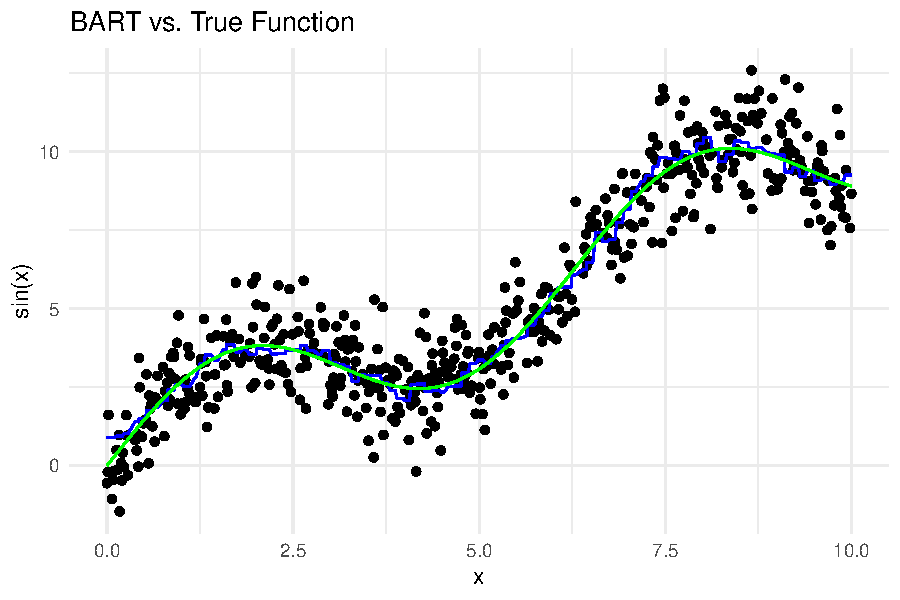
\includegraphics[width=0.7\textwidth]{outputs/sin_plot.pdf}
  \caption{Plot of the estimates (blue) against observations (black) and generating function(green)}
  \label{plot_sin1}
\end{figure}

To check convergence of the posterior, we plot in figure \ref{plot_sin2} the posterior draws of $\sigma$, the uniquely identified parameter, including the burn-in period (at the left of the red line). We observe that the MCMC draw converges quickly to the true parameter. after a burn-in period of 100 iterations, although the draws oscillate with some autocorrelation due to the posterior sampling procedure, which generates dependent samples.

\begin{figure}[h]
  \centering
  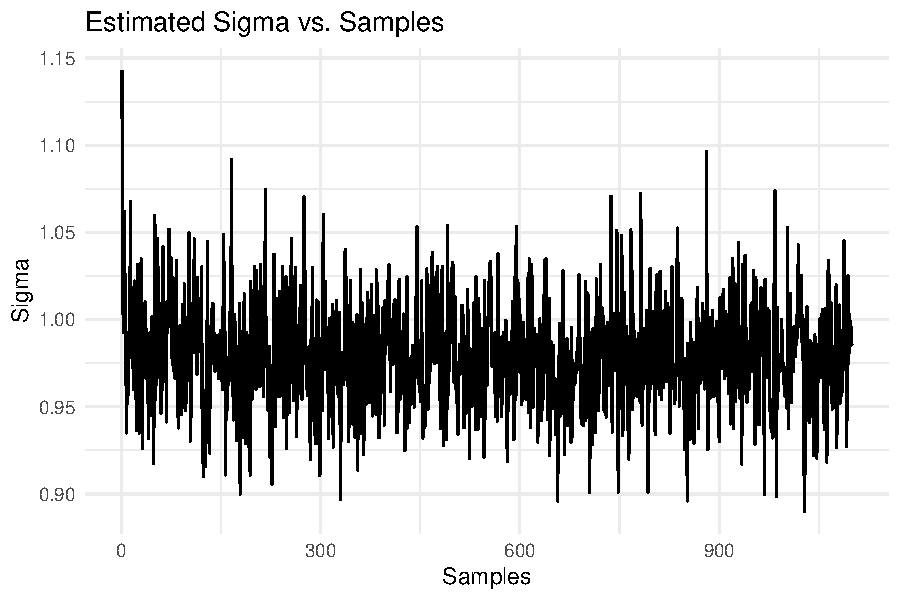
\includegraphics[width=0.7\textwidth]{outputs/sigma_plot.pdf}
  \caption{Value of $\sigma$ over MCMC iterations}
  \label{plot_sin2}
\end{figure}


To check robustness of BART to different prior specifications, we consider different values for the prior mean of $\sigma$: 100, 0.001 and 1 (the true one). With $\sigma = 100$ (the blue line), we observe in plot \ref{plot_sin3} underfitting of the data, because the prior is telling to BART that a large part of the variation is due to the idiosyncratic error $\varepsilon$ in \eqref{likelihood}. A small $\sigma$, like $\sigma = 0.001$ (the red line), should in theory push BART to overfit the training set. However, from the graph \ref{plot_sin3}, it is clear that the regularization prior is still strong enough to avoid the overfitting. The green line corresponds instead to BART estimated with the true population $\sigma$.

\begin{figure}[h]
  \centering
  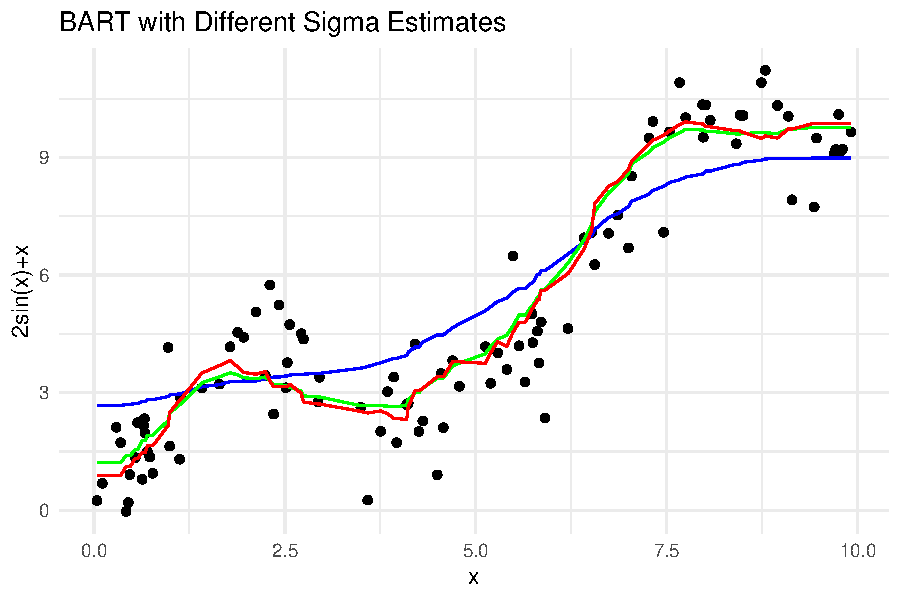
\includegraphics[width=0.7\textwidth]{outputs/sin_plot_diff_sigma.pdf}
  \caption{Different prior mean of $\sigma$}
  \label{plot_sin3}
\end{figure}


\subsection{Predicting the age of an Abalone}

Abalone are marine snails from the family \textit{Haliotidae}, which are found in various regions around the world. Determining their age is a labor-intensive process, as it requires cutting through the shell, staining it, and then counting the growth rings under a microscope. However, predicting the age of an abalone can also be done by examining other physical characteristics of the individual, which are much easier to assess. This is precisely the motivation behind our application.

We use Abalone characteristics data coming from the UC Irvine Machine Learning Repository \parencite{warwicknashAbalone1994a}, described in table \ref{table1}. Our dataset contains 4177 observations with no missing values. No data manipulation is necessary, aside from creating a new variable, \( \text{Age} = \text{Rings} + 1.5 \), and removing the column identifying the number of rings. 

\begin{table}[h]
  \centering
  \begin{tabular}{llllll}

  \toprule
  Variable Name & Role & Type & Description & Units \\
  \midrule
  Sex                  & Feature       & Categorical   & M, F, and I (infant) & -    \\
  Length               & Feature       & Continuous    & Longest shell measurement & mm\\
  Diameter             & Feature       & Continuous    & Perpendicular to length & mm  \\
  Height               & Feature       & Continuous    & With meat in shell      & mm  \\
  Whole\_weight         & Feature       & Continuous    & Whole abalone           & gram\\
  Shucked\_weight       & Feature       & Continuous    & Weight of meat          & gram\\
  Viscera\_weight       & Feature       & Continuous    & Gut weight (after bleeding) & \\
  Shell\_weight         & Feature       & Continuous    & After being dried       & gram\\
  Rings                & Target        & Integer       & +1.5 gives the age in years & - \\

   \bottomrule
  \end{tabular}
  \caption{Table of Variables}
  \label{table1}
  \end{table}
Our target variable $y$ in this dataset is represented by Age. Our $p = 8$ covariates are the ones labelled as "Feature" in table \ref{table1}.

Our aim is to compare the predictive performance of the different tree ensemble models discussed in theory in the sections above. We thus run BART from \cite{mccullochBARTBayesianAdditive2024}; Boosting from \cite{ridgewayGbmGeneralizedBoosted2024}; Random Forest and Bagging from \cite{breimanRandomForestBreimanCutlers2024}. 
Notice that since BART adopts a Bayesian framework, it is able to provide a measure of the uncertantiy regarding its prediction, while other frequentist methods cannot. Indeed, BART allows to show boxplots of the posterior samples of predictions. Figure \ref{fig:bart_box} displays the boxplots of the draws of $\hat{y}$ (on the $y$-axis) ordered by the average predicted age (on the $x$-axis).

\begin{figure}[h]
    \centering
    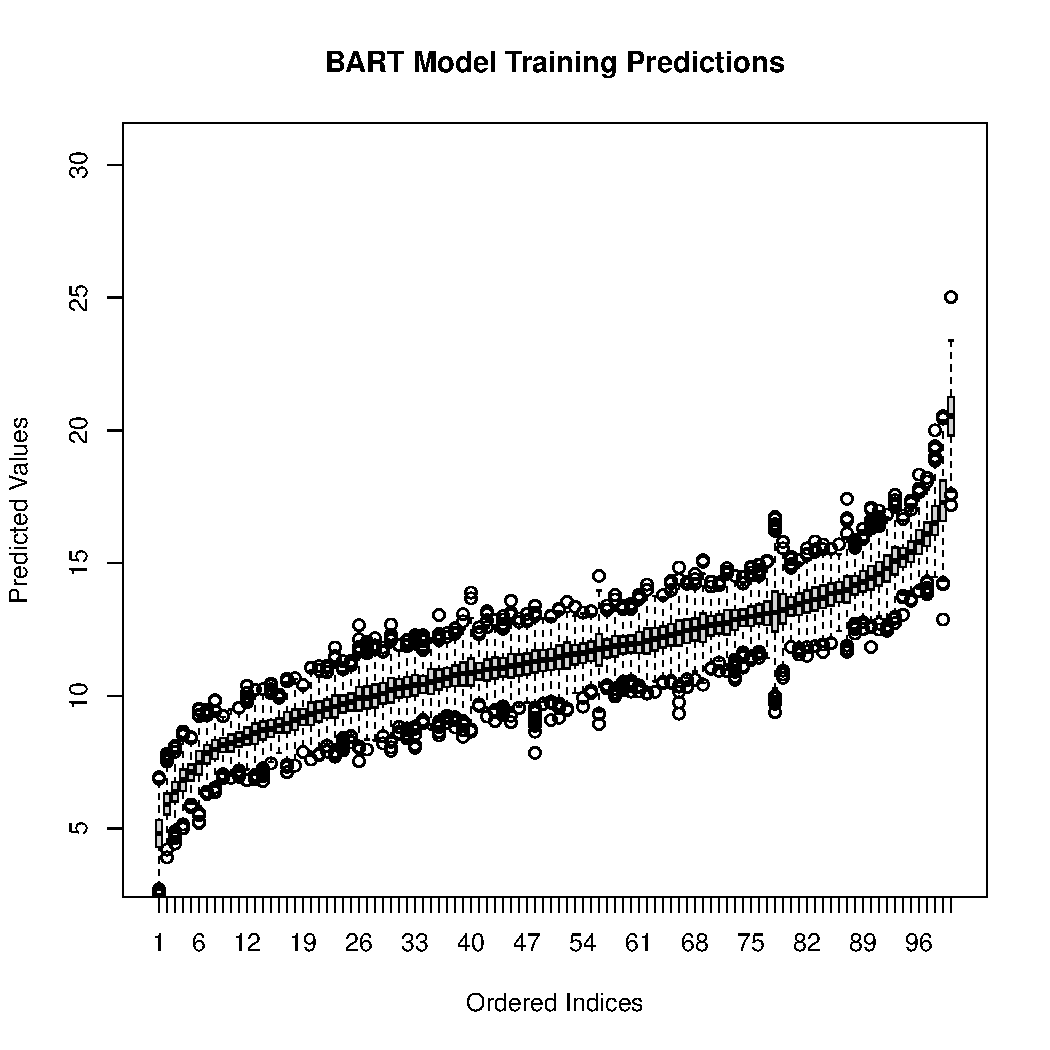
\includegraphics[width=0.7\linewidth]{outputs/bart_boxplot.pdf}
    \caption{Ordered boxplot of BART estimates}
    \label{fig:bart_box}
\end{figure}




In order to assess the predictive performance of the models, we divide the sample set in half: a training set used to fit  $\hat{y}$ (predicted age), and a testing set to compute the out of bag Mean Squared Errors (MSE) for predicting the same variable. We use the classic formula for the MSE, 
\[\text{MSE} = \frac{1}{n} \sum_{i=1}^{n} (y_i - \hat{y}_i)^2
\]
Models are run for various values of $m$, the number of trees, and for each value, both the mean squared error (MSE) of out-of-sample predictions and the computation time are recorded.

Table \ref{table2} displays the MSE and the computation time for all the tree ensemble models with the number of trees equal to 500. Consistently to what was showed by \cite{chipmanBARTBayesianAdditive2010} for 42 different datasets, the performance of BART in terms of MSE is comparable or even slightly superior to that of other tree ensemble methods. However, since BART is a Bayesian method, it requires time-consuming MCMC iterations for posterior inference, even in the default prior setting. This increases the time needed for BART to be run relative to the other models.
\begin{table}[h]
  \centering
  \begin{tabular}{lcc}
  \toprule
  Model           & MSE & Time (s) \\
  \midrule
  BART            & 4.45    & 66.7  \\
  Random Forest   & 4.53    & 4.74  \\
  Boosting        & 4.87    & 0.220 \\
  Bagging         & 4.54    & 12.4  \\
  \bottomrule
  \end{tabular}
  \caption{Model performance with $m=500$} \label{table2}
  \end{table}






The same findings hold when we let the number of trees vary. In Figure \ref{plot_mse}, we see that the MSE for BART is lower than that of the other models, but it quickly stabilizes after 500 trees, similarly to the other models. It is worth noting that boosting, which in theory should be the frequentist model more similar to BART, has a significantly higher MSE for all numbers of trees, probably due to ineffective parameter tuning.
\begin{figure}[h]
  \centering
  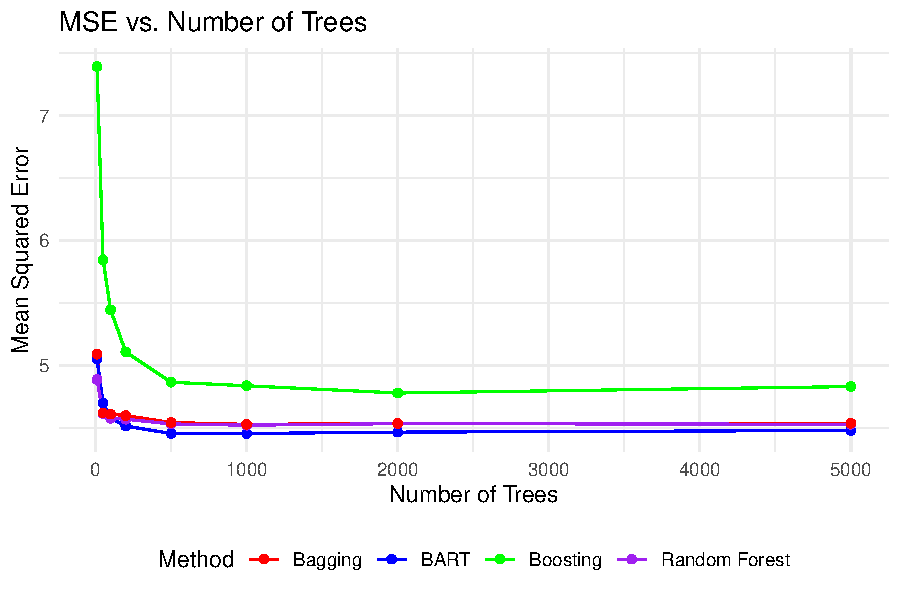
\includegraphics[width=0.7\textwidth]{outputs/mse_plot.pdf}
  \caption{Mean Squared Error for different values of $m$}
  \label{plot_mse}
\end{figure}

Figure \ref{plot_time} displays the number of seconds needed for the model to converge. Although it is the best performer, BART is also the model that takes the longest to be run, and computation time scales linearly with the number of trees that are fitted.
\begin{figure}[h]
  \centering
  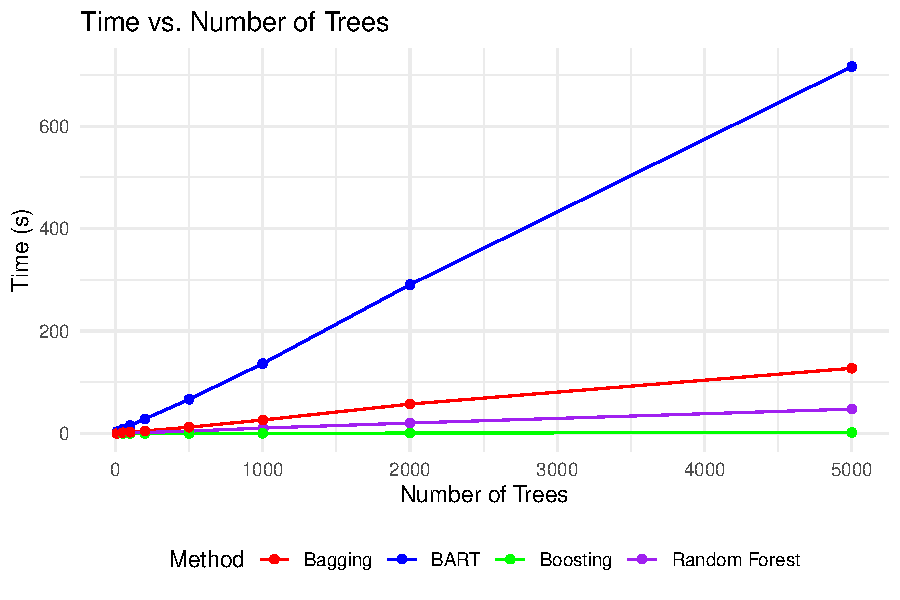
\includegraphics[width=0.7\textwidth]{outputs/time_plot.pdf}
  \caption{Time of computations for different values of $m$}
  \label{plot_time}
\end{figure}


\section{Conclusion}
\label{conclusion}
BART is a Bayesian sum-of-trees model that exploits a regularization prior to constrains each tree to be a weak learner. Fitting and posterior inference is perfomed via a MCMC algorithm that combines Gibbs and Metropolis-Hastings. Since the parameter space of BART has unbounded dimension, BART is a nonparametric model, that is a Bayesian model on an infinite-dimensional
parameter space. BART chooses the dimension of the parameter space $ (\{T_j, M_j\}_{j=1}^m, \sigma^2) $ depending on the sample, such that the effective complexity of the model (as measured by the
number of dimensions used) adapts to the data. In particular, each tree is allowed to change in its number of decision rules and leaves. 
The Bayesian setting of BART allows posterior inference including point and interval estimates of the unknown regression function $f(\mathbf{x})$. 

The data application shows that the theoretical features of BART (the prior and the posterior inference algorithm) influence its predictive performance compared to other ensembe methods. In particular, the necessity of doing MCMC iterations in order to fit the model implies that BART requires more computation time respect to Random Forests, Bagging, and Boosting. However, the flexibility due to the fact that it is a nonparamtric Bayesian model allows it to perform well even in the default setting, i.e. using the default hyperparameters of \texttt{gbart}.
 
 In the simulation experiment, BART obtained posterior
 mean and interval estimates of the true responde variable $\hat{y}$. BART's performance was robust to different hyperparameter specifications, for example different choices of prior $\sigma$. In the Abalone dataset, BART was able to perform reliable age prediction for Abalone shells given other features.


\section{Acknowledgments}
LLMs were used in this project for checking clarity and grammar of the initial drafted version, specifically in the introduction and abstract part. Moreover, were used to improve and check the correctness of the R-code. The LLMs used were ChatGPT, Claude and Github Copilot.


\newpage

\printbibliography




\end{document}
